\begin{exercise}\label{ex:02-01-5periodic-cayley} Show that a pair of   ellipses $x^2/A^2+y^2/B^2=1$ and $x^2/a^2+y^2/b^2=1$ with semi-axes $(A,B)$ and $(a,b)$ ($A>a,\;B>b$) has a porism of pentagons (5-periodic orbits) then
\[\frac{a^3}{A^3}+\frac{b^3}{B^3}+\left(\frac{a}{A}+\frac{b}{B}\right)^2=1+\left(\frac{a}{A}+\frac{b}{B}\right)\left(1+\frac{ab}{AB}\right)\]\end{exercise}

\begin{exercise}\label{ex:02-02-quarticcurve} Consider a quartic curve $q(x,y)=x^4+y^4-1=0$ and a family of circles $\mathcal{C}_r:  \; x^2+y^2-r^2=0$.

\noindent i) Determine $r$ such that there is  1d-family of triangles inscribed in the quartic $x^4+y^4=1$ and sides tangent to the circle $x^2+y^2=r^2$. Analyze   properties of this family of triangles. See   \cref{fig:darbouxq4c2}.

\noindent ii) Show that the square with vertices $[\pm \frac{1}{\sqrt[4]{2}},\pm \frac{1}{\sqrt[4]{2}}]$ is inscribed in $ q(x,y)=0$ and its sides are tangent to the circle $x^2+y^2=\frac{\sqrt{2}}{2}.$ In this case show that there is no porism of Poncelet associated to the algebraic curves. See \cref{fig:period4darboux}.

\begin{figure}[H]
    \centering
    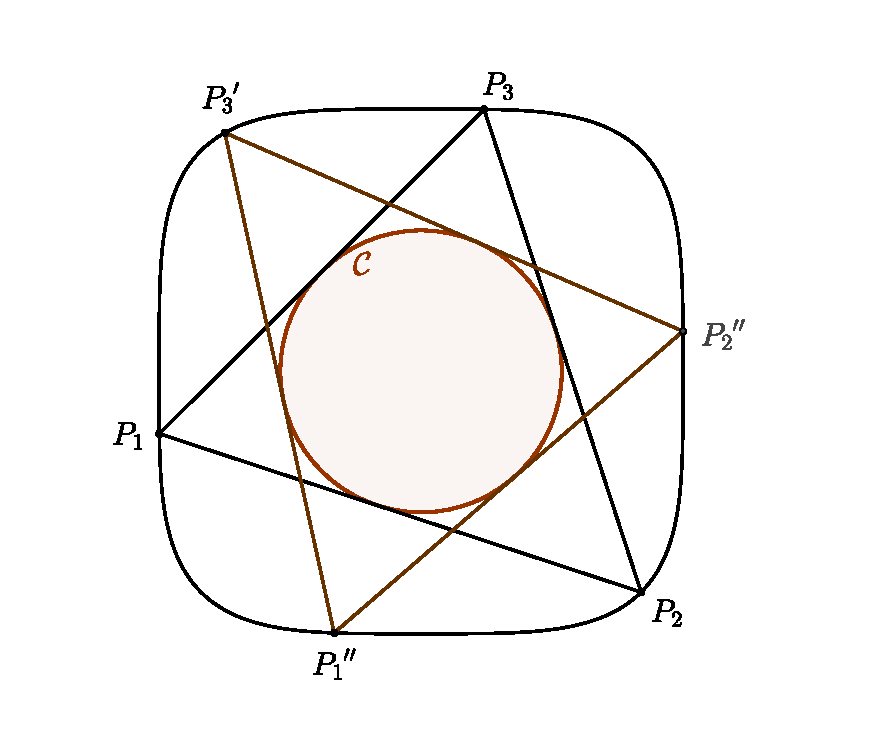
\includegraphics[scale=0.4]{pics_02_035_darboux_Q4_C2.pdf}
    \caption{Porism of triangular orbits in a pair of a quartic and a circle.}
    \label{fig:darbouxq4c2}
\end{figure}


\begin{figure}
    \centering
     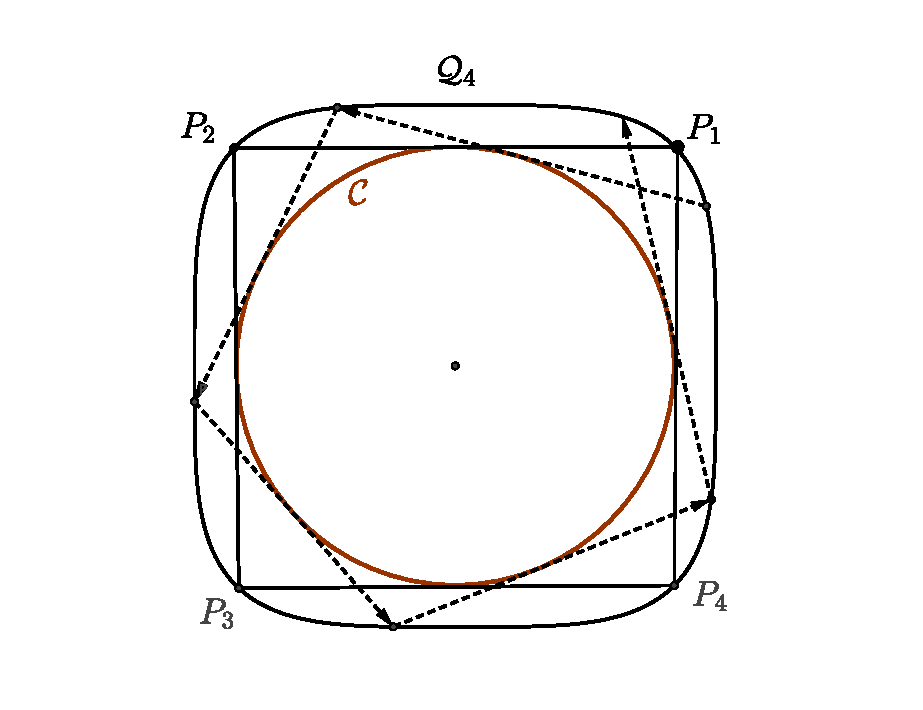
\includegraphics[scale=0.4]{pics_02_040_periodo4_darboux_Q4_C2.pdf}
    \caption{Non existence of a porism of quadrilateral orbits in a pair of a quartic $\mathcal{Q}_4$ and a circle $\mathcal{C}$.}
    \label{fig:period4darboux}
\end{figure}

\end{exercise}
\begin{exercise}\label{exer:02-03-ponceletpair}
Show that the ellipse $x^2/a^2+y^2/b^2=1$ and the circle $(x+c)^2+y^2=4a^2$ define  a Poncelet pair such that  all  orbits have   period 3.
\end{exercise}

\begin{exercise}\label{exer:02-04-ponceletpair-center}
Consider a triangle $T$ given by three lines $\ell_i$ $(i=1,2,3)$. 

\noindent i) Show that given a point $M$ in the interior of $T$ there exists an ellipse (or hyperbola) centered at $M$ and tangent to the lines $\ell_i$.

\noindent ii) Show that when $M$ is in the interior of medial triangle of $T$ the conic of item i) is an ellipse.

\noindent iii) Construct an ellipse centered at $M$ and passing through the vertices of $T$. Conclude that in the conditions of item ii) we obtain a concentric pair of ellipses having $T$ as 3-periodic of the Poncelet pair.

\end{exercise}

\begin{exercise}\label{ex:23} 

\end{exercise}


\begin{exercise}\label{ex:24}

\end{exercise}